\documentclass{article} 

\usepackage[english]{babel}
\usepackage{polynom}
\usepackage{tikz}
\usepackage{amsmath}
\usepackage{amsfonts}
\usepackage{cancel}
\usepackage{pgfplots}
\usepackage{xcolor}
\usepackage{listings}
\usepackage{hyperref}
\usepackage{enumitem}
\usepackage{titlesec}
\usepackage{comment}
\pgfplotsset{width=10cm, compat=1.18}
\title{MATH1851 Part 1}
\author{Victor Chui}
\begin{document}
\maketitle
\tableofcontents
\pagebreak

\section{1011 Knowledge Revisit}
\subsection{Limit at 0, infinity}
\subsubsection{Limit at 0}
It is common to see $\lim_{x \to 0} f(x)$ or $\lim_{x \to \infty} f(x)$
in most of the limit questions.\\\\ This section will particularly state the cases with 0 and infinity,
and state their respective answers for better understanding.\\
\\First, for limit at 0:
\begin{equation}
  \lim_{x \to 0^+} \frac{1}{x} = \infty
\end{equation}
\begin{equation} \label{eq:2} 
  \lim_{x \to 0^-} \frac{1}{x} = -\infty
\end{equation}
\begin{equation} \label{eq:3}
  \lim_{x \to 0} \frac{1}{x} = undefined
\end{equation}
The above could be proved just by substituting numbers. Try substitute 0.5 and 0.05 in equation 1.
As you can see, the number becomes larger as it approaches to 0.\\
\\For equation 2, try substitute -0.05 and -0.5. The number becomes smaller as it approaches to 0. \\\\
However, since the limit of $0^+$ and $0^-$ are not equal, that means $\lim_{x \to 0} \frac{1}{x}$ does not exist hence undefined.
\\
\\Now, onto infinity.
\subsubsection{Limit at infinity}
Define the following limit.
\begin{equation*}
  \lim_{x \to \infty} \frac{f(x)}{g(x)} 
\end{equation*}
Given three kinds of limit equations below:
\begin{equation} \label{eq:1}
  \lim_{x \to \infty} \frac{5x-3}{6x^2+11}
\end{equation}
\begin{equation} \label{eq:2}
  \lim_{x \to \infty} \frac{5x^2-3}{6x^2+11}
\end{equation}
\begin{equation} \label{eq:3}
  \lim_{x \to \infty} \frac{5x^3-3}{6x^2+11}
\end{equation}
Consider equation $(4)$,
\begin{equation*}
  \lim_{x \to \infty} \frac{5x-3}{6x^2+11}
\end{equation*}
We know that since the degree of the denominator is more dominant, which we can pull to the case that $\lim_{x \to \infty} \frac{1}{x} = 0$.
\\\\
Consider equation $(5)$,
\begin{equation*}
  \lim_{x \to \infty} \frac{5x^2-3}{6x^2+11}
\end{equation*}
We know that since the maximum degree of both the numerator and the demoniator are equal, therefore we could just take the coefficient of their maximum degree and return the answer. In this case, $\lim_{x \to \infty} \frac{5}{6} = \frac{5}{6}$
\\\\
Consider equation $(6)$,
\begin{equation*}
  \lim_{x \to \infty} \frac{5x^3-3}{6x^2+11}
\end{equation*}
We know that the degree of the numerator is more dominant, which we can pull to the case that $\lim_{x \to \infty} 5x = \infty$.
\subsubsection{Special cases}
Case 1:
\begin{equation*}
  \lim_{x \to \alpha} \frac{x}{\infty} = 0
\end{equation*}
Case 2:
\begin{equation*}
  \lim_{x \to \alpha} \frac{x}{0} = \infty
\end{equation*}
Note that in this case $\alpha$ can be $\infty$.\\
\subsection{Area of a curve}
Given $y = f(x)$, $y = g(x)$, where $f(x) > g(x)$.
The area of the curves bounded by f(x) and g(x) is going to be:
\begin{equation*}
  A = \int_{a}^{b} f(x)-g(x)dx
\end{equation*}
In other words, when f(x) is on top of g(x), then we can use this formula (top - bottom).
\\\\
Given $x = f(y)$, $x = g(y)$, where $f(y) > g(y)$.
The area of the curves bounded by f(y) and g(y) is going to be:
\begin{equation*}
  A = \int_{c}^{d} f(y)-g(y)dx
\end{equation*}
In other words, when f(x) is on the right side of g(x), we can use this formula. (right - left)
\begin{comment}
\begin{center}
\begin{tikzpicture}
\begin{axis}[
    axis lines = left,
    xlabel = \(x\),
    ylabel = {\(y\)},
]
%Below the red parabola is defined
\addplot [
    domain=-10:10, 
    samples=100, 
    color=red,
]
{x^2 -4*x};
\addlegendentry{\(x^2 + 2x + 1\)}
%\draw (axis cs:2,0) -- node[left]{Text} (axis cs:2,20);

\end{axis}
\end{tikzpicture}
\end{center}
\end{comment}

\subsection{Rationalisation}
\section{Theorems}
\subsection{Mean Value Theorem}
\subsection{Extreme Value Theorem}
\section{More Limits}
\subsection{Two sides limits}
\subsubsection{Definition of a limit which exist}
A limit is considered defined and exist when
\begin{equation*}
  \lim_{x \to a^+} f(x) = \lim_{x \to a^-} f(x) 
\end{equation*}
\subsection{Continuity}
\subsubsection{Definition}
For a function $f(x)$ to be continuous, we need to satisfy the following two conditions:
\begin{equation*}
  \text{1. }\lim_{x \to a} f(x) = f(a)
\end{equation*}
\begin{equation*}
  \text{2. }f(a)\text{ is defined.}
\end{equation*}
\subsubsection{Continuity Test}
As section 3.1 already mentioned that for a limit two exist, we have to examine both the left hand limit (-) and the right hand limit (+). Thus, we can test the continuity by the following steps.
$$
\text{1. Find if }\lim_{x \to a^+} f(x) == \lim_{x \to a^-} f(x) \text{.}
$$
$$
\text{2. Find the value of }f(a)\text{.}
$$
Then we can check whether the three values are the same. If they are, then it is continous. If not, then it is a discontinuous function.
\subsubsection{Intermediate Value Theorem}
The definition of IVT are as follows.
$$
\text{If a function f(x) is proven as continuous at interval }[a,b]\text{,}
$$
$$
\text{let M be any numbers which lies between f(a) and f(b)}
$$
$$
\text{then there is a number c such that }c \in [a,b] \text{ and }f(c) = M \text{.}
$$
\subsection{Differentiability}
We have discussed the continuity of a function in Section 3.2. Now, we will talk about differentiability, which is crucial in part 1.
\subsubsection{Definition}
The definition of differentiability is as follows.
$$
\text{1. }\lim_{h \to 0} \frac{f(c+h)-f(x)}{h} \text{ should be defined (except 0 and infinity) at every c when }c \in [a,b]\text{.}
$$
$$
\text{2. The function should be continuous.}
$$
We know that if a function is differentiable, then it \textbf{MUST} be continuous. It doesn't mean that the function is differentiable when it is continuous.
\subsubsection{Special case}
For one to be continuous but not differentiable, the slope at a point should be undefined. A few common examples are listed below.


1. Sharp turns (which the slope at the transition point is parallel to the x-axis).


2. Vertical tangents (the slope of a vertical line is undefined)

\subsection{L'Hopital Rule}
\subsubsection{Application}
L'Hopital Rule should be applied when you encounter the following situation:
\begin{equation*}
  \lim_{x \to a} \frac{\infty} {\infty} \text{ or } \lim_{x \to a} \frac{0}{0}
\end{equation*}
Note that you can't use this rule when $\infty * 0$.
\subsubsection{Techniques}
You can use L'Hospital Rule when you can construct the following condition(s):
$$
\lim_{x \to a} \frac{\frac{1}{0}} {\infty}
$$
\section{Differentiation}
\subsection{Fundamental Theorem of Calculus}
\subsubsection{Definition}
\section{Integration}
\subsection{Techniques for Trigonometric Integration}
Consider the following equation of trigonometric integration.
\begin{equation*}
  I = \int \sin^m(x) \cos^n(x)
\end{equation*}
There are two general cases to solve this type of questions. If m and/or n are odd, then it is case 1. If both of them are even, then it is case 2.
\subsubsection{Case 1: Any Odds}
Consider the following equation below:
\begin{equation*}
  \int \cos^3(2x) \sin^5(2x)
\end{equation*}
We have to factor out one of them, so we will take factor of $\cos(2x)$ as the factor.
\begin{equation*}
  \int \cos(2x) \cos^2(2x) \sin^5(2x)
\end{equation*}
Recall
\begin{equation*}
  \frac{d\sin(2x)}{dx} = 2\cos(2x)
\end{equation*}
We can let $u = \sin(2x)$ and write down the expression.
\begin{equation*}
  \frac{1}{2} \int (1-u^2)u^5 
\end{equation*}
Then, we can use the power rule to solve the integral.
\begin{equation*}
  \frac{1}{2} (\frac{\cos^6(2x)}{6} - \frac{\cos^8(2x)}{8})
\end{equation*}
\subsubsection{Case 2: Both even}
For both even, we can use double-angle formula to help us.
Recall (Provided in the exam paper)
\begin{equation}
  \sin(2A) = 2\sin(A)\cos(A)
\end{equation}
\begin{equation}
  \cos(2x) = 1-2\sin^2(x) = 2\cos^2(x)-1
\end{equation}
Just use this formula everytime we see even degree in trigonometry. Let's demonstrate with an example.\\
Given the formula
\begin{equation*}
  \int \sin^4(x) \cos^4(x) \text{dx}
\end{equation*}
In this equation, we can generalize the equation, such as:
\begin{equation*}
  \int (\sin(x) \cos(x))^4 \text{dx}
\end{equation*}
Using double angle identities, we have:
\begin{equation*}
  \frac{1}{16} \int \sin^4(2x) \text{dx}
\end{equation*}
We just keep using the double angle identities until the very end.
\begin{equation*}
  \frac{1}{16} \int (\sin^2(2x))^2 \text{dx}
\end{equation*}
\begin{equation*}
  \frac{1}{64} \int (1-\cos(4x))^2 \text{dx}
\end{equation*}
\begin{equation*}
  \frac{1}{64} \int 1-2\cos(4x)+\cos^2(4x) \text{dx}
\end{equation*}
We perform double angle identities on $\cos^2(4x)$ again,
\begin{equation*}
  \frac{1}{64} \int 1-2\cos(4x)+\frac{1}{2}(1+\cos(8x)) \text{dx}
\end{equation*}
The solved integral is
\begin{equation*}
  \frac{3x}{128}-\frac{\sin(4x)}{128}+\frac{\sin(8x)}{1024}+C 
\end{equation*}
\subsubsection{Case 3: Others}
There are two cases for solving the other types of trigonometry. Given the two integral below:
\begin{equation*}
  \int \tan^{m}x \sec^{n}x \text{dx}
\end{equation*}
\begin{equation*}
  \int \cot^{m}x \csc^{n}x \text{dx}
\end{equation*}
We can follow the two rules below: \\
If $\tan$ or $\cot$ is odd, then we factor out $\sec x\tan x$ or $\csc x \cot x$ in the identity, and use the formula $\tan^2 x = \sec^2 x-1$ or $\cot^2 x = \csc^2 x -1$. \\
If $\sec$ or $\csc$ is even, then we keep $\sec^2 x$ or $\csc^2 x$ and use the formula $\sec^2 = \tan^2+1$ or $\csc^2 = \cot^2+1$.
\subsubsection{Example}
Let's try out a few example.
\begin{equation*}
  \int \cot^5 x \csc^5 x \text{dx}
\end{equation*}
Since $\cot$ is odd, we try to take out the form $\csc x \cot x$.
\begin{equation*}
  \int \cot^4 x \csc^4 x (\cot x\csc x) \text{dx}
\end{equation*}
\begin{equation*}
  \int (\cot^2 x)^2 \csc^4 x (\cot x\csc x) \text{dx}
\end{equation*}
Let $u = \csc x$. Then, $du = -\csc x \cot x dx$.
\begin{equation*}
  -\int (u^2-1)^2 u^4 \text{du}
\end{equation*}
Solving this as a normal integration, then it is solvable.\\
Let's look at another question.
\begin{equation*}
  \int \tan^3 x \text{dx}
\end{equation*}
Since $\tan$ is odd,
\begin{equation*}
  \int \frac{\tan^2 x}{\sec x} \tan x\sec x \text{dx}
\end{equation*}
Let $u = secx$, $du = \tan x\sec x \text{dx}$
\begin{equation*}
  \int \frac{u^2 -1} {u} \text{du}
\end{equation*}
\begin{equation*}
  \int u \text{du} - \int \frac{1}{u} \text{du}
\end{equation*}
Solve this as normal integral.
\\Let's look at another example.
\begin{equation*}
  \int \sec^4 x \tan^2 x \text{dx}
\end{equation*}
Since $\sec$ is even, 
\begin{equation*}
  \int (\sec^2 x)^2 \tan^2 x \text{dx}
\end{equation*}
Let $u = \tan x$, $du = \sec^2 x \text{dx}$.
\begin{equation*}
  \int (u^2+1)u^2 \text{du}
\end{equation*}
\subsection{Trigonometric Substitution}
All sorts of trigonometric substitution can be found by a right-angled triangle using Pythagoras Theorem.
\\
Given the integral:
\begin{equation*}
  \int \sqrt{a^2-x^2} \text{dx}
\end{equation*}
We can try to find the substitution for x.\\
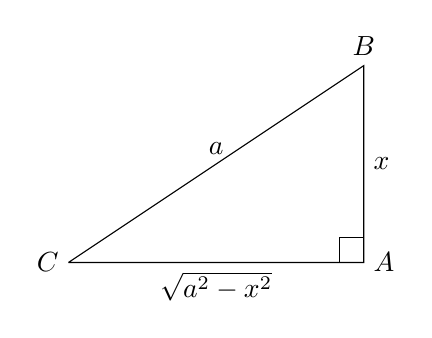
\begin{tikzpicture}[scale=1.25]%,cap=round,>=latex]

\coordinate [label=left:$C$] (A) at (-1.5cm,-1.cm);
\coordinate [label=right:$A$] (C) at (1.5cm,-1.0cm);
\coordinate [label=above:$B$] (B) at (1.5cm,1.0cm);
\draw (A) -- node[above] {$a$} (B) -- node[right] {$x$} (C) -- node[below] {$\sqrt{a^2-x^2}$} (A);
\draw (1.25cm,-1.0cm) rectangle (1.5cm,-0.75cm);
\end{tikzpicture}
\\In all the following figures, let $\theta =\angle C$.
\\
In our trigonometric formula, we must include x.
\begin{equation*}
  \sin \theta = \frac{x}{a} 
\end{equation*}
\begin{equation*}
  x = a\sin \theta
\end{equation*}
Let us consider another type of integral. 
\begin{equation*}
  \int \sqrt{x^2-a^2} \text{dx}
\end{equation*}
Consider the triangle below:\\ 
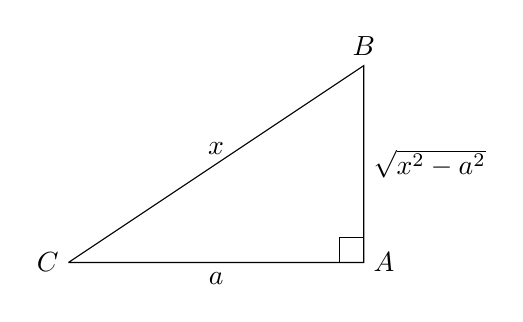
\begin{tikzpicture}[scale=1.25]%,cap=round,>=latex]
\coordinate [label=left:$C$] (A) at (-1.5cm,-1.cm);
\coordinate [label=right:$A$] (C) at (1.5cm,-1.0cm);
\coordinate [label=above:$B$] (B) at (1.5cm,1.0cm);
\draw (A) -- node[above] {$x$} (B) -- node[right] {$\sqrt{x^2-a^2}$} (C) -- node[below] {$a$} (A);
\draw (1.25cm,-1.0cm) rectangle (1.5cm,-0.75cm);
\end{tikzpicture}
\\Then, we can find out the relation in this triangle.
\begin{equation*}
  \sec \theta = \frac{x}{a}
\end{equation*}
\begin{equation*}
  x = a\sec \theta
\end{equation*}
Lastly, let us consider the last type of integral which we can use trigonometric substitution.
\begin{equation*}
  \int \sqrt{a^2+x^2} \text{dx}
\end{equation*}
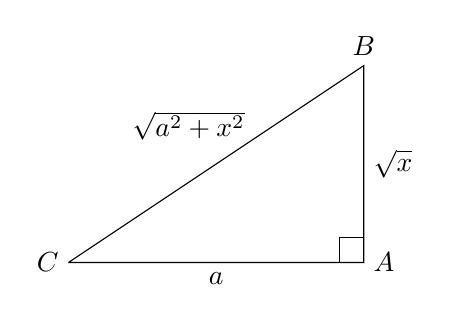
\begin{tikzpicture}[scale=1.25]%,cap=round,>=latex]
  \coordinate [label=left:$C$] (A) at (-1.5,-1);
  \coordinate [label=right:$A$] (C) at (1.5,-1.0);
  \coordinate [label=above:$B$] (B) at (1.5,1.0);
  \draw (A) -- node[above, pos=0.5, anchor=east, left=10, above=5] {$\sqrt{a^2+x^2}$} (B) -- node[right, pos=0.5] {$\sqrt{x}$} (C) -- node[below, pos=0.5] {$a$} (A);
  \draw (1.25,-1.0) rectangle (1.5,-0.75);
\end{tikzpicture}
\\Then, we can find out the relation in this triangle.
\begin{equation*}
  \tan \theta = \frac{x}{a}
\end{equation*}
\begin{equation*}
  x = a\tan \theta
\end{equation*}
\subsection{Partial Fractions}
The reason why partial fractions exist here is solely because Laplace Transform (Covered in 1851 part 2).\\
Let's begin.
\subsubsection{Case 1: Normal cases}
To perform Partial Fractions, the highest degree of the numerator must be smaller than the denominator. Here's an example.
\begin{equation*}
  \frac{7x-23}{(x-2)(x-5)}
\end{equation*}
As the below equation shown, the denominator has the highest degree of 2.\\
Now, based on the above example, let's solve this partial fraction problem.
We break down this fractions into parts, such that:
\begin{equation*}
  \frac{7x-23}{(x-2)(x-5)} = \frac{A}{x-2} + \frac {B}{x-5}
\end{equation*}
Notice that for the variables on the numerator, it should be one degree less than the denominator. (Covered in later parts)\\
Multiply both sides by $(x-2)(x-5)$.
\begin{equation*}
  7x-23 = A(x-5) + B(x-2)
\end{equation*}
Substitute x = 5 or x = 2 to solve the equation. Then we get a partial fraction form.
\begin{equation*}
  \frac{7x-23}{(x-2)(x-5)} = \frac{3}{x-2} + \frac{4}{x-5}
\end{equation*}
\subsubsection{Case 2: Degree condition is not satisfied}
Now, if the degree of the numerator is higher or equal than the degree of the denominator, we perform long divison. Below is an example.
\begin{equation*}
  \frac{x^2+3x-1}{(x+1)(x-2)}
\end{equation*}
Then, we can perform long division.\\
\begin{center}
\polylongdiv{x^2+3x-1}{x^2-x-2}
\end{center}
The following fractions can be written as below.
\begin{equation*}
  \frac{x^2+3x-1}{(x+1)(x-2)} = 1 + \frac{4x+1}{(x+1)(x-2)}
\end{equation*}
\subsubsection{Case 3: Repeated Roots in denominator}
\begin{equation*}
  \frac{2x-5}{x^2(x+1)}
\end{equation*}
We have to do the following.
\begin{equation*} 
  \frac{2x-5}{x^2(x+1)} = \frac{A}{x} + \frac{B}{x^2} + \frac{C}{x+1}
\end{equation*}
Notice that the reason the second fraction isn't Bx+C is that we have to follow the lower degree, which in this case it is A.
\subsection{Volume of Solid}
For the area between an interval, the area is added by individual small rectangle inside the graph, which the area of the respective rectangle is
\begin{equation*}
  A_1 = f(x) * \Delta x
\end{equation*}
which $f(x)$ is the height of the rectangle, and $\Delta x$ is the width.\\
If we have 10 rectangles to sum up as the area, then we have the following:
\begin{equation*}
  A_{10} = \sum_{k=1}^{10} f(x_k) * \Delta x
\end{equation*}
Thus, if we have infinite number of rectangles, we have:
\begin{equation*}
  A = \lim_{n\to \infty} \sum_{k=1}^{n} f(x_k) * \Delta x
\end{equation*}
Thus, it could be rewritten to:
\begin{equation*}
  A = \int_{a}^{b} f(x) dx
\end{equation*}
\subsubsection{Disk Method}
Notice that in any cylindrical volume at any shape, the cross section given is a circle.\\
By defintion of an area, 
\begin{equation*}
  V(x) = A(x) * l
\end{equation*}
which $A(x)$ is the cross-sectional area, and $l$ is the length of the cylindar.
\section{Parametric Equations (Optional)}
\subsection{Definition}
\subsection{Arc Length}
\subsection{Surface Area of Revolution}
\subsection{Example}
\end{document}
